% ===== pca =====
\section*{Principal Component Analysis (PCA)}

\subsection*{What PCA Does}
\textbf{Goal:} reduce unlabeled data from $D$ to $k \ll D$ dimensions (e.g.\ 10{,}000 $\rightarrow$ 100) while losing as little information as possible.

\subsection*{PCA Step by Step}

\begin{keeptogether}
\textbf{Running example} (2D $\rightarrow$ 1D): 6 points $(0,0),(0,1),(1,0),(1,2),(2,1),(2,2)$. The cloud stretches along a diagonal.

{\centering
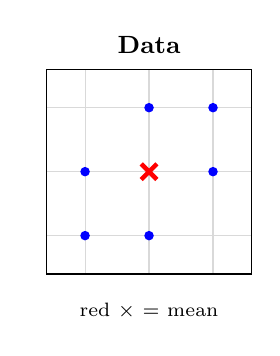
\begin{tikzpicture}
\begin{axis}[scale only axis, width=2.6cm, height=2.6cm, enlargelimits=false,
    grid=major, grid style={gray!30}, major tick length=0pt,
    xticklabels={}, yticklabels={}, title style={yshift=-4pt}, label style={font=\scriptsize},
    xmin=-0.6, xmax=2.6, ymin=-0.6, ymax=2.6,
    title={\small\textbf{Data}}, xlabel={\scriptsize red $\times$ = mean}]
\addplot[only marks, mark=*, blue, mark size=1.5pt] coordinates {(0,0) (0,1) (1,0) (1,2) (2,1) (2,2)};
\addplot[only marks, mark=x, red, mark size=4pt, ultra thick] coordinates {(1,1)};
\end{axis}
\end{tikzpicture}
\par}
\end{keeptogether}

\begin{keeptogether}
\textbf{Step 1: Center.} Subtract the mean from every point (the best line passes through the mean):
\[
\bar{\mathbf{x}} = \frac1N\sum_{n=1}^N \mathbf{x}_n = (1,1),
\qquad
\mathbf{x}_n \leftarrow \mathbf{x}_n - \bar{\mathbf{x}}
\]

{\centering
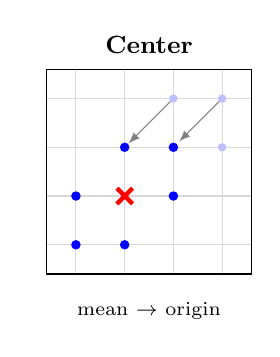
\begin{tikzpicture}
\begin{axis}[scale only axis, width=2.6cm, height=2.6cm, enlargelimits=false,
    grid=major, grid style={gray!30}, major tick length=0pt,
    xticklabels={}, yticklabels={}, title style={yshift=-4pt}, label style={font=\scriptsize},
    xmin=-1.6, xmax=2.6, ymin=-1.6, ymax=2.6,
    title={\small\textbf{Center}}, xlabel={\scriptsize mean $\rightarrow$ origin}]
\addplot[only marks, mark=*, blue!25, mark size=1.3pt] coordinates {(0,0) (0,1) (1,0) (1,2) (2,1) (2,2)};
\addplot[gray, -latex] coordinates {(2,2) (1.12,1.12)};
\addplot[gray, -latex] coordinates {(1,2) (0.08,1.08)};
\addplot[only marks, mark=*, blue, mark size=1.5pt] coordinates {(-1,-1) (-1,0) (0,-1) (0,1) (1,0) (1,1)};
\addplot[only marks, mark=x, red, mark size=4pt, ultra thick] coordinates {(0,0)};
\end{axis}
\end{tikzpicture}
\par}
\end{keeptogether}

\begin{keeptogether}
\textbf{Step 2: Find the eigenvectors.} Stack the centered points as rows of $X$. The eigenvectors of $X^\top X$ are the cloud's long and short axes:
\[
X^\top X = \begin{bmatrix}4&2\\2&4\end{bmatrix},
\qquad
\mathbf{u}_1 = \tfrac{1}{\sqrt2}(1,1),\; \lambda_1 = 6,
\qquad
\mathbf{u}_2 = \tfrac{1}{\sqrt2}(1,-1),\; \lambda_2 = 2
\]

{\centering
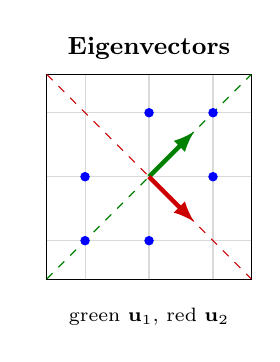
\begin{tikzpicture}
\begin{axis}[scale only axis, width=2.6cm, height=2.6cm, enlargelimits=false,
    grid=major, grid style={gray!30}, major tick length=0pt,
    xticklabels={}, yticklabels={}, title style={yshift=-4pt}, label style={font=\scriptsize},
    xmin=-1.6, xmax=1.6, ymin=-1.6, ymax=1.6,
    title={\small\textbf{Eigenvectors}}, xlabel={\scriptsize green $\mathbf{u}_1$, red $\mathbf{u}_2$}]
\addplot[green!50!black, dashed, domain=-1.6:1.6, samples=2] {x};
\addplot[red!80!black, dashed, domain=-1.6:1.6, samples=2] {-x};
\addplot[only marks, mark=*, blue, mark size=1.5pt] coordinates {(-1,-1) (-1,0) (0,-1) (0,1) (1,0) (1,1)};
\addplot[green!50!black, ultra thick, -latex] coordinates {(0,0) (0.707,0.707)};
\addplot[red!80!black, ultra thick, -latex] coordinates {(0,0) (0.707,-0.707)};
\end{axis}
\end{tikzpicture}
\par}
\end{keeptogether}

\begin{keeptogether}
\textbf{Step 3: Keep the top $k$.} Each eigenvalue is the spread along its eigenvector, so keep the largest. Here $k = 1$: keep $\mathbf{u}_1$ ($\lambda_1 = 6$), drop $\mathbf{u}_2$ ($\lambda_2 = 2$). \textbf{Fraction of variance kept} $= \frac{\lambda_1 + \dots + \lambda_k}{\lambda_1 + \dots + \lambda_D}$, here $\frac{6}{8} = 75\%$.

{\centering
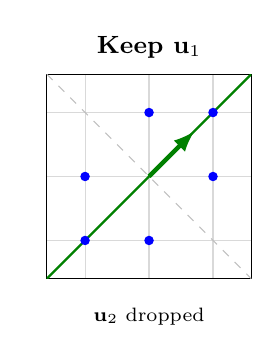
\begin{tikzpicture}
\begin{axis}[scale only axis, width=2.6cm, height=2.6cm, enlargelimits=false,
    grid=major, grid style={gray!30}, major tick length=0pt,
    xticklabels={}, yticklabels={}, title style={yshift=-4pt}, label style={font=\scriptsize},
    xmin=-1.6, xmax=1.6, ymin=-1.6, ymax=1.6,
    title={\small\textbf{Keep $\mathbf{u}_1$}}, xlabel={\scriptsize $\mathbf{u}_2$ dropped}]
\addplot[green!50!black, thick, domain=-1.6:1.6, samples=2] {x};
\addplot[gray!50, dashed, domain=-1.6:1.6, samples=2] {-x};
\addplot[only marks, mark=*, blue, mark size=1.5pt] coordinates {(-1,-1) (-1,0) (0,-1) (0,1) (1,0) (1,1)};
\addplot[green!50!black, ultra thick, -latex] coordinates {(0,0) (0.707,0.707)};
\end{axis}
\end{tikzpicture}
\par}
\end{keeptogether}

\begin{keeptogether}
\textbf{Step 4: Project.} Drop each point onto the $\mathbf{u}_1$ line at a right angle. It becomes how far along $\mathbf{u}_1$ it lands, one number per point:
\[
z_n = \mathbf{x}_n^\top \mathbf{u}_1,
\qquad \text{e.g.\ } (1,1) \rightarrow \tfrac{1+1}{\sqrt2} = \sqrt2
\]
Result: $z = -\sqrt2,\, -\tfrac{1}{\sqrt2},\, -\tfrac{1}{\sqrt2},\, \tfrac{1}{\sqrt2},\, \tfrac{1}{\sqrt2},\, \sqrt2$.

{\centering
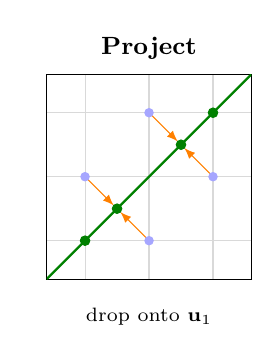
\begin{tikzpicture}
\begin{axis}[scale only axis, width=2.6cm, height=2.6cm, enlargelimits=false,
    grid=major, grid style={gray!30}, major tick length=0pt,
    xticklabels={}, yticklabels={}, title style={yshift=-4pt}, label style={font=\scriptsize},
    xmin=-1.6, xmax=1.6, ymin=-1.6, ymax=1.6,
    title={\small\textbf{Project}}, xlabel={\scriptsize drop onto $\mathbf{u}_1$}]
\addplot[green!50!black, thick, domain=-1.6:1.6, samples=2] {x};
\addplot[orange, -latex] coordinates {(-1,0) (-0.55,-0.45)};
\addplot[orange, -latex] coordinates {(0,-1) (-0.45,-0.55)};
\addplot[orange, -latex] coordinates {(0,1) (0.45,0.55)};
\addplot[orange, -latex] coordinates {(1,0) (0.55,0.45)};
\addplot[only marks, mark=*, blue!35, mark size=1.5pt] coordinates {(-1,0) (0,-1) (0,1) (1,0)};
\addplot[only marks, mark=*, green!50!black, mark size=1.7pt] coordinates {(-1,-1) (-0.5,-0.5) (0.5,0.5) (1,1)};
\end{axis}
\end{tikzpicture}
\par}
\end{keeptogether}

\begin{keeptogether}
\textbf{Step 5 (if asked): Reconstruct.} Start at the mean and go $z_n$ along $\mathbf{u}_1$. The gap $\mathbf{x}_n - \hat{\mathbf{x}}_n$ is the error:
\[
\hat{\mathbf{x}}_n = \bar{\mathbf{x}} + z_n\,\mathbf{u}_1
\]

{\centering
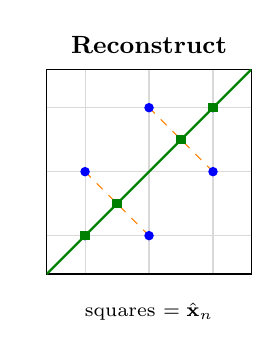
\begin{tikzpicture}
\begin{axis}[scale only axis, width=2.6cm, height=2.6cm, enlargelimits=false,
    grid=major, grid style={gray!30}, major tick length=0pt,
    xticklabels={}, yticklabels={}, title style={yshift=-4pt}, label style={font=\scriptsize},
    xmin=-0.6, xmax=2.6, ymin=-0.6, ymax=2.6,
    title={\small\textbf{Reconstruct}}, xlabel={\scriptsize squares $= \hat{\mathbf{x}}_n$}]
\addplot[green!50!black, thick, domain=-0.6:2.6, samples=2] {x};
\addplot[orange, dashed] coordinates {(0,1) (0.5,0.5)};
\addplot[orange, dashed] coordinates {(1,0) (0.5,0.5)};
\addplot[orange, dashed] coordinates {(1,2) (1.5,1.5)};
\addplot[orange, dashed] coordinates {(2,1) (1.5,1.5)};
\addplot[only marks, mark=*, blue, mark size=1.5pt] coordinates {(0,0) (0,1) (1,0) (1,2) (2,1) (2,2)};
\addplot[only marks, mark=square*, green!50!black, mark size=1.5pt] coordinates {(0,0) (0.5,0.5) (1.5,1.5) (2,2)};
\end{axis}
\end{tikzpicture}
\par}
\end{keeptogether}

\begin{keeptogether}
\subsection*{Why the Top Eigenvector}
PCA picks the unit direction $\mathbf{u}$ that keeps the most spread:
\[
\max_{\|\mathbf{u}\|=1} \; \sum_{n=1}^N (\mathbf{x}_n^\top\mathbf{u})^2 = \max_{\|\mathbf{u}\|=1}\; \mathbf{u}^\top X^\top X\,\mathbf{u}
\quad\Longrightarrow\quad
X^\top X\,\mathbf{u} = \lambda\mathbf{u}
\]

{\centering
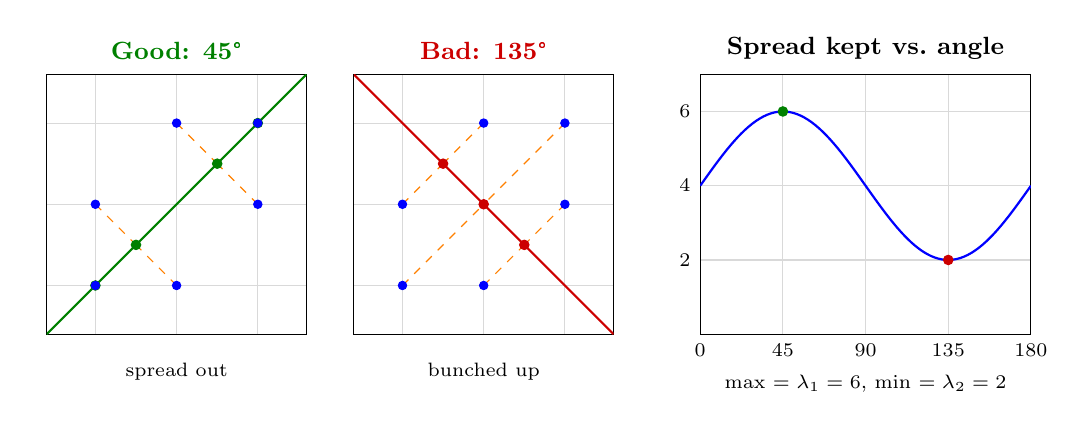
\begin{tikzpicture}
\begin{axis}[name=g,
    scale only axis, width=3.3cm, height=3.3cm,
    xmin=-1.6, xmax=1.6, ymin=-1.6, ymax=1.6, enlargelimits=false,
    grid=major, grid style={gray!30}, major tick length=0pt,
    xticklabels={}, yticklabels={},
    title={\small\textbf{Good: 45°}}, title style={text=green!50!black, yshift=-4pt},
    xlabel={\scriptsize spread out}, label style={font=\scriptsize}]
\addplot[green!50!black, thick, domain=-1.6:1.6, samples=2] {x};
\addplot[orange, dashed] coordinates {(-1,0) (-0.5,-0.5)};
\addplot[orange, dashed] coordinates {(0,-1) (-0.5,-0.5)};
\addplot[orange, dashed] coordinates {(0,1) (0.5,0.5)};
\addplot[orange, dashed] coordinates {(1,0) (0.5,0.5)};
\addplot[only marks, mark=*, green!50!black, mark size=1.7pt] coordinates {(-1,-1) (-0.5,-0.5) (0.5,0.5) (1,1)};
\addplot[only marks, mark=*, blue, mark size=1.5pt] coordinates {(-1,-1) (-1,0) (0,-1) (0,1) (1,0) (1,1)};
\end{axis}
\begin{axis}[name=h, at={(g.east)}, anchor=west, xshift=0.6cm,
    scale only axis, width=3.3cm, height=3.3cm,
    xmin=-1.6, xmax=1.6, ymin=-1.6, ymax=1.6, enlargelimits=false,
    grid=major, grid style={gray!30}, major tick length=0pt,
    xticklabels={}, yticklabels={},
    title={\small\textbf{Bad: 135°}}, title style={text=red!80!black, yshift=-4pt},
    xlabel={\scriptsize bunched up}, label style={font=\scriptsize}]
\addplot[red!80!black, thick, domain=-1.6:1.6, samples=2] {-x};
\addplot[orange, dashed] coordinates {(-1,-1) (0,0)};
\addplot[orange, dashed] coordinates {(1,1) (0,0)};
\addplot[orange, dashed] coordinates {(-1,0) (-0.5,0.5)};
\addplot[orange, dashed] coordinates {(0,1) (-0.5,0.5)};
\addplot[orange, dashed] coordinates {(0,-1) (0.5,-0.5)};
\addplot[orange, dashed] coordinates {(1,0) (0.5,-0.5)};
\addplot[only marks, mark=*, red!80!black, mark size=1.7pt] coordinates {(0,0) (-0.5,0.5) (0.5,-0.5)};
\addplot[only marks, mark=*, blue, mark size=1.5pt] coordinates {(-1,-1) (-1,0) (0,-1) (0,1) (1,0) (1,1)};
\end{axis}
\begin{axis}[at={(h.east)}, anchor=west, xshift=1.1cm,
    scale only axis, width=4.2cm, height=3.3cm,
    xmin=0, xmax=180, ymin=0, ymax=7, enlargelimits=false,
    grid=major, grid style={gray!30}, major tick length=0pt,
    xtick={0,45,90,135,180}, ytick={2,4,6},
    tick label style={font=\scriptsize},
    title={\small\textbf{Spread kept vs.\ angle}}, title style={yshift=-4pt},
    xlabel={\scriptsize max $= \lambda_1 = 6$, min $= \lambda_2 = 2$}, label style={font=\scriptsize}]
\addplot[thick, blue, domain=0:180, samples=90] {4 + 2*sin(2*x)};
\addplot[only marks, mark=*, green!50!black, mark size=1.7pt] coordinates {(45,6)};
\addplot[only marks, mark=*, red!80!black, mark size=1.7pt] coordinates {(135,2)};
\end{axis}
\end{tikzpicture}
\par}

\begin{itemize}
  \item \textbf{Max spread = min error.} length$^2$ = kept$^2$ + lost$^2$ (Pythagoras), so kept + lost $= 8$ at every angle.
  \item \textbf{Eigenvalue = spread} along its eigenvector, so keep the largest $\lambda$'s.
\end{itemize}
\end{keeptogether}
